\section{Tuning Parameter on LAS Scores}

For given treebanks \(A\) and \(B\), we defined \(\theta_{LAS}\) in Definition \ref{def:harmony} as
\begin{equation*}
        \theta_{LAS} = \vert {LAS}_{x,x} - {LAS}_{y,x} \vert \hspace{5mm} \quad \forall [x, y \in \{A,B\}] \tag{\ref{eq:deprel_harmony}}
\end{equation*}
where \(LAS_{P,Q}\) indicates LAS when trained on \(P\) and tested on \(Q\).

A few properties of the metric \(\theta_{LAS}\) can be mentioned here.
\begin{enumerate}
    \item In an ideal scenario, the metric \(\theta_{LAS}\) should not be negative. Since we are training and evaluating on the same dataset, we expect \({LAS}_{x,x}\) to be considerably high. In case a treebank has a lower score when trained and tested on itself, either the parsing algorithm fails to capture the linguistic data (verifiable by training and evaluating on treebanks of same language, if possible), or the annotation procedure is very likely to be non-uniform across the given treebank. The latter can also be because of the different genres of data present therein.
    \item The exact value of the metric is the greater value of the two associations. Simply speaking, if treebanks P, and Q are being evaluated, the maximal value from either of P or Q being evaluated on the other becomes the metric score.
    \item In general, the lower the value of the metric, the better.
\end{enumerate}
    
In this section, we shall try to optimize \(\theta_1\) value, given \(\theta_{LAS}\) values for different treebanks as given in Table \ref{tab:harmony_las_confusion}, reported in form of confusion matrices as in \cite{alonso2016universal}. The horizontal rows mark the treebank the parser was trained on, while the vertical column marks the treebank on which the parser was tested. Following a look at the \(\theta_{LAS}\) values, we try to address the different factors that might affect the metric value. Eventually, we try to find the optimal value range for \(\theta_1\) in order for the considered treebanks to be considered harmonious with each other, with respect to \(\theta_1\) parameter.

\newpage

\begin{table}[H]
    \begin{minipage}{.45\linewidth}
    \begin{tabular}{|l|l|l|}
    \hline
    \verb|es| & AnCora & GSD \\
    \hline
    AnCora & 86.36 & 68.07 \\
    \hline
    GSD & 68.81 & 85.30 \\
    \hline
    \end{tabular}%
    \vspace{5mm}
    \begin{tabular}{|l|l|l|}
    \hline
    \verb|et| & EDT & EWT \\
    \hline
    EDT & 85.19 & 75.60 \\
    \hline
    EWT & 72.76 & 92.35 \\
    \hline
    \end{tabular}%
    \vspace{5mm}
    \begin{tabular}{|l|l|l|}
    \hline
    \verb|fi| & FTB & TDT \\
    \hline
    FTB & 92.30 & 48.65 \\
    \hline
    TDT & 52.17 & 87.78 \\
    \hline
    \end{tabular}%
    \vspace{5mm}
    \begin{tabular}{|l|l|l|}
    \hline
    \verb|gl| & CTG & TreeGal \\
    \hline
    CTG & 82.02 & 25.27 \\
    \hline
    TreeGal & 56.67 & 90.97 \\
    \hline
    \end{tabular}%
    \vspace{5mm}
    \begin{tabular}{|l|l|l|}
    \hline
    \verb|grc| & Perseus & PROIEL \\
    \hline
    Perseus & 70.54 & 43.23 \\
    \hline
    PROIEL & 32.02 & 75.84 \\
    \hline
    \end{tabular}%
    \vspace{5mm}
    \begin{tabular}{|l|l|l|}
    \hline
    \verb|ko| & GSD & Kaist \\
    \hline
    GSD & 63.95 & 28.07 \\
    \hline
    Kaist & 32.76 & 72.27 \\
    \hline
    \end{tabular}%
    \vspace{5mm}
    \begin{tabular}{|l|l|l|}
    \hline
    \verb|lt| & ALKSNIS & HSE \\
    \hline
    ALKSNIS & 90.02 & 51.66 \\
    \hline
    HSE & 47.26 & 88.98 \\
    \hline
    \end{tabular}%
    \end{minipage}%
    \begin{minipage}{.5\linewidth}
    \begin{tabular}{|l|l|l|}
    \hline
    \verb|nl| & Alpino & LassySmall \\
    \hline
    Alpino & 88.10 & 79.06 \\
    \hline
    LassySmall & 76.56 & 92.34 \\
    \hline
    \end{tabular}%
    \vspace{5mm}
    \begin{tabular}{|l|l|l|}
    \hline
    \verb|pl| & LFG & PDB \\
    \hline
    LFG & 98.72 & 67.10 \\
    \hline
    PDB & 84.11 & 88.13 \\
    \hline
    \end{tabular}%
    \vspace{5mm}
    \begin{tabular}{|l|l|l|}
    \hline
    \verb|pt| & Bosque & GSD \\
    \hline
    Bosque & 87.91 & 63.63 \\
    \hline
    GSD & 36.67 & 88.67 \\
    \hline
    \end{tabular}%
    \vspace{5mm}
    \begin{tabular}{|l|l|l|}
    \hline
    \verb|ro|\footnote{Annotated Data not in correct CONLL-U format, UD Parser not trainable or testable on the data} & Nonstandard & RRT \\
    \hline
    Nonstandard & 00.00 & 00.00 \\
    \hline
    RRT & 00.00 & 84.49 \\
    \hline
    \end{tabular}%
    \vspace{5mm}
    \begin{tabular}{|l|l|l|}
    \hline
    \verb|sl| & SSJ & SST \\
    \hline
    SSJ & 94.43 & 56.01 \\
    \hline
    SST & 71.82 & 88.07 \\
    \hline
    \end{tabular}%
    \vspace{5mm}
    \begin{tabular}{|l|l|l|}
    \hline
    \verb|sv| & LinES & Talbanken \\
    \hline
    LinES & 91.37 & 74.50 \\
    \hline
    Talbanken & 76.05 & 91.99 \\
    \hline
    \end{tabular}%
    \vspace{5mm}
    \begin{tabular}{|l|l|l|l|}
    \hline
    \verb|fr| & GSD & ParTUT & Sequoia\\
    \hline
    GSD & 91.07 & 78.99 & 78.17 \\
    \hline
    ParTUT & 78.38 & 96.12 & 77.32 \\
    \hline
    Sequoia & 78.59 & 78.23 & 93.85 \\
    \hline
    \end{tabular}
    \end{minipage}%
\end{table}%
\begin{table}[H]
\begin{tabular}{|l|l|l|l|}
    \hline
    \verb|la| & ITTB & Perseus & PROIEL \\
    \hline
    ITTB & 86.29 & 38.34 & 39.38 \\
    \hline
    Perseus & 29.18 & 77.34 & 38.53 \\
    \hline
    PROIEL & 35.83 & 34.12 & 75.82 \\
    \hline
    \end{tabular}
    \vspace{5mm}
    \newline
    \begin{tabular}{|l|l|l|l|}
    \hline
    \verb|ru| & GSD & SynTagRus & Taiga\\
    \hline
    GSD & 90.56 & 70.62 & 61.85 \\
    \hline
    SynTagRus & 73.55 & 86.59 & 67.22 \\
    \hline
    Taiga & 70.02 & 69.75 & 84.62 \\
    \hline
    \end{tabular}%
    \vspace{5mm}
    \newline
    \begin{tabular}{|l|l|l|l|}
    \hline
    \verb|no| & Bokmaal & Nynorsk & NynorskLIA \\
    \hline
    Bokmaal & 91.47 & 82.27 & 61.20 \\
    \hline
    Nynorsk & 85.26 & 91.12 & 62.01 \\
    \hline
    NynorskLIA & 69.79 & 68.66 & 89.03 \\
    \hline
    \end{tabular}%
    \vspace{5mm}
    \newline
    %Level 4
    \begin{tabular}{|l|l|l|l|l|}
    \hline
    \verb|cs| & CAC & CLTT & FicTree & PDT \\
    \hline
    CAC & 85.25 & 72.57 & 80.78 & 78.55 \\
    \hline
    CLTT & 68.92 & 93.83 & 64.40 & 63.64 \\
    \hline
    FicTree & 74.20 & 69.51 & 92.30 & 74.25 \\
    \hline
    PDT & 81.61 & 76.21 & 83.15 & 84.85 \\
    \hline 
    \end{tabular}%
    \vspace{5mm}
    \newline
    \begin{tabular}{|l|l|l|l|l|}
    \hline
    \verb|en| & EWT & GUM & LinES & ParTUT \\
    \hline
    EWT & 88.29 & 77.06 & 75.56 & 70.30 \\
    \hline
    GUM & 76.36 & 91.48 & 75.50 & 71.39 \\
    \hline
    LinES & 70.41 & 69.81 & 90.83 & 67.05 \\
    \hline 
    ParTUT & 66.70 & 68.25 & 69.79 & 94.09 \\
    \hline 
    \end{tabular}%
    \vspace{5mm}
    \newline
    \begin{tabular}{|l|l|l|l|l|}
    \hline
    \verb|it| & ISDT & ParTUT & PoSTWITA & VIT\\
    \hline
    ISDT & 90.10 & 88.48 & 64.79 & 79.22 \\ 
    \hline
    ParTUT & 84.72 & 94.18 & 62.40 & 76.94 \\
    \hline
    PoSTWITA & 81.71 & 81.71 & 84.83 & 75.33 \\
    \hline
    VIT & 82.57 & 82.25 & 63.26 & 86.26 \\
    \hline
    \end{tabular}%
    
    \caption{LAS Scores (in \%) for Different Treebanks per language, UDv2.4}Parsed with GS Tokenisation with GS Tags
    \label{tab:harmony_las_confusion}
\end{table}

A couple of inferences can be made quite clearly from the data, wherein we see how the performance of the parser model is affected with respect to treebanks. If we look at \verb|ko| parser scores, we can see that the parsers perform rather poorly as compared to other treebanks when training and testing data remains the same. This is very likely because of the treebanks not following consistent annotation scheme within itself.

We have almost discounted for the size of the data by selecting the treebanks with some training data available, but not entirely. Consider the case of \verb|cs| treebanks for example. The token counts of the train data in different treebanks for \verb|cs| is as shown in Table \ref{tab:cs_size}. Owing to smaller training data, the parser trained on \verb|cs|-CLTT data performs the poorest among the parsers in the language. At the same time, due to larger training data, the parser performs the best when trained on PDT data. Therefore, we need to still regulate for train data size disparities.

\begin{table}[H]
    \centering
    \begin{tabular}{l|l|l|}
        Treebank & Sentences & Tokens\\
        \hline
        CAC & 23 478 & 471 594\\
        CLTT & 860 & 26 225\\
        FicTree & 10 160 & 133 137\\
        PDT & 68 495 & 1 171 190\\
    \end{tabular}%
    \caption{train Size of cs Treebanks}
    \label{tab:cs_size}
\end{table}
    
If we take a look at the sub-table containing LAS scores for parsers in \verb|fi|, the two parsers perform unsatisfactorily on the other treebank. However, looking at the data in Table \ref{tab:fi_size}, we can safely discount the effect of size disparity as the sole reason for the low performance. Looking at the GitHub repositories for the two treebanks\footnote{\url{https://github.com/UniversalDependencies/UD_Finnish-FTB}}\footnote{\url{https://github.com/UniversalDependencies/UD_Finnish-TDT}}, and the base reference for TDT Treebank \citep{Haverinen2014}, we can understand the genre distribution in the two treebanks, as listed in Table \ref{tab:fi_genera}.

\begin{table}[H]
    \begin{minipage}{0.4\linewidth}
    \begin{tabular}{l|l}
        Treebank & Sentence Counts \\
        \hline
        FTB & 14 981 \\
        TDT & 12 217 \\
    \end{tabular}%
    \caption{train Size of fi Treebanks}
    \label{tab:fi_size}
    \end{minipage}%
    \quad
    \begin{minipage}{0.5\linewidth}
    \begin{tabular}{l|l}
        Treebank & Genres \\
        \hline
        FTB & grammar-examples \\
        TDT & news, wiki, blog, \\
        & legal, fiction, \\
        & grammar-examples \\
    \end{tabular}%
    \caption{Genres in fi Treebanks}
    \label{tab:fi_genera}
    \end{minipage}
\end{table}

Notice that while the TDT Treebank contains multiple genres, FTB is composed of a singular genre. In sub-section \ref{ssec:genre_theta2}, we study the effect of genre classification with respect to parser performances. It is worth noting that while the genre classification can easily be done in case of some treebanks (as in case of \verb|fi| above), it might not always be possible to do so.

\subsection{Optimization for Size Disparity}
\label{ssec:size_theta1}

To properly account for size disparities, we need to keep in mind two aspects, as listed:

\begin{enumerate}
    \item The data is homogenous in nature. By homogenous, we mean that the data should be crawled from same or very similar sources. Also, the term also implies that the data should be from a singular genre so that genre based fluctuations do not affect the scores.
    \item We should have sufficient data available, so as to be able to compare the different sized splits, and their relative performances.
\end{enumerate}

\verb|hi|-hdtb treebank is one of the treebanks that satisfies both the above conditions. The treebank's split of train, test and dev data is as shown in Table \ref{tab:hi_size}. As an additional data reference, we use news section of \verb|hi|-pud. The size of the splits of the PUD treebanks in general, is as shown in Table \ref{tab:hi_pud_size}.

\begin{table}[H]
    \begin{minipage}{.45\linewidth}
    \centering
    \begin{tabular}{l|l}
    Split & Sentence Counts \\
    \hline
    dev & 1 659 \\
    test & 1 684 \\
    train & 13 304 \\
    \end{tabular}
    \caption{Size of hi-hdtb treebank}
    \label{tab:hi_size}
    \end{minipage}%
    \begin{minipage}{.50\linewidth}
    \centering
    \begin{tabular}{l|l}
    Category & Sentences \\
    \hline
    News & 500 \\
    Wiki & 500 \\
    \hline
    Total & 1 000 \\
    \end{tabular}
    \caption{Sentences in PUD treebanks}
    \label{tab:hi_pud_size}
    \end{minipage}
\end{table}

We process the train data of \verb|hi|-hdtb in a workflow, defined as follows:
\begin{enumerate}
    \item Split the data into sizes in the range of \{5, 10, ..., 95\} \% of the original data size.
    \item On the split data, train a UDPipe Parser for the split, with the dev data given as heldout, and report the scores on \verb|hi|-hdtb test data, as well as news section of \verb|hi|-pud.
    \item Report the LAS Scores in a graphical format.
\end{enumerate}

\begin{figure}[H]
    \centering
    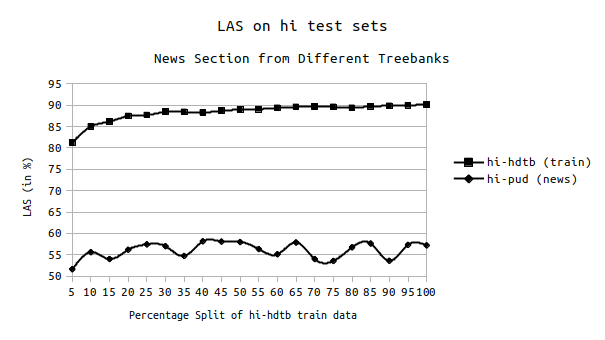
\includegraphics[scale=0.90]{img/size-theta1-1}
    \caption{LAS for size disparity}
    \label{fig:size-theta1-1}
\end{figure}

The graph in Figure \ref{fig:size-theta1-1} shows two curves that demonstrate the performance of the parser as the training data increases in size. In case of \verb|hi|-hdtb train data, the splits until around 12.6\% are less than the size of the test data. That is marked clearly in the graph as the lowest performance score by the parser. As the split size increases, and thus the number of training instances, the parser performs better and better, the performance increasing monotonically.

In case of \verb|hi|-pud news section, even at 5\%, the size of training data exceeds the size of test data. However, the parser performance is significantly lower than on \verb|hi|-hdtb test data. Also, unlike the previous curve, the performance is largely varying, with multiple local minima.

Even though the data belongs to the same genre in the two testing sets, there is considerable difference between the two. In the case of \verb|hi|-hdtb data, the dataset is crawled from newspaper dailies, and thus contains news articles, as they were printed. In the case of \verb|hi|-pud news section though, the data was originally in either of English, German, French, Italian or Spanish, and they were translated to Hindi by using English as pivot language. Thus, there are instances where the nuance of the original language might be lost, since the news reporting style in the two languages is not very often similar.

Nonetheless, we can make some general statements about the performance by looking at the given data. We notice that based on the available data for training, the performance of the parser can vary as much as 10\% when on the same data (i.e. data belonging to same documents as well).

Since the parser performance starts saturating at different points, we can describe the saturating points in the form of size factors, and how the LAS score can be affected when considering the effect of size alone. We give a formula for the upper bound of the difference in metrics based on size first, and then illustrate it with an example.

\theoremstyle{definition}
\begin{definition}
\label{def:theta1_size}
    Given two treebanks, \(A\) and \(B\), with \(\alpha\) as the size ratio of the treebanks when measured in terms of number of tokens in the train data, we can bound \(\theta_{LAS}\) by an upper bound given by \(\theta_{1, size}\) as below.
    \begin{equation*}
        size(A) \geq size(B) \implies \alpha = \frac{size(A)}{size(B)}
    \end{equation*}
    \begin{equation}
    \theta_{1, size} = 
    \begin{cases}
         \frac{min(10, \zeta)}{32} + \frac{\gamma}{16} + \frac{\epsilon}{8} + \frac{\delta}{4} + \frac{\beta}{2} & \text{if } \theta_{LAS} > 1\\
        1 & otherwise
    \end{cases}
    \end{equation}
    where \(\zeta = \lfloor\alpha - 80\rfloor \text{, \quad} \gamma = \lfloor\alpha - \zeta - 60\rfloor \leq 20 \text{, \quad} \epsilon = \lfloor\alpha - \zeta - \gamma - 40\rfloor \leq 20 \text{, \quad} \delta = \lfloor\alpha - \zeta - \gamma - \epsilon - 20\rfloor \leq 20 \text{, \quad} \beta = \lfloor\alpha-\zeta-\gamma-\epsilon-\delta\rfloor \leq 20 \text{, \quad}\beta\text{, }\delta\text{, }\epsilon\text{, }\gamma\text{, }\zeta \geq 0\)
\end{definition}

\begin{example}
We are given two treebanks, containing the same genre of data, differing in the size. Let us assume the two given parameters as follows, with the size given in terms of tokens in train data:
\begin{gather*}
    size(A) = 1 200 000 \text{tokens in train data}\\
    size(B) = 10 000 \text{tokens in train data}\\
    \alpha = 120\\
    LAS(A,A) = 92\\
    LAS(A,B) = 65\\
    LAS(B,B) = 91
    LAS(B,A) = 75\\
    \theta_{LAS} = max(92-65, 91-75) = max(27, 16) = 27
\end{gather*}

We can estimate the upper bound on \(\theta_{LAS}\) as follows:
\begin{gather*}
\zeta = \lfloor\alpha - 80\rfloor = \lfloor120-80\rfloor = \lfloor40\rfloor = 40\\
\gamma = \lfloor\alpha - \zeta - 60\rfloor = \lfloor120-40-60\rfloor = \lfloor20\rfloor = 20\\
\epsilon = \lfloor\alpha - \zeta - \gamma -40\rfloor = \lfloor120-20-20-40\rfloor = \lfloor20\rfloor = 20\\
\delta = \lfloor\alpha - \zeta - \gamma - \epsilon - 20\rfloor = \lfloor120-40-20-20-20\rfloor = \lfloor20\rfloor = 20\\
\beta = \lfloor\alpha-\zeta-\gamma-\epsilon-\delta\rfloor = \lfloor120-40-20-20-20\rfloor = \lfloor20\rfloor = 20\\
\theta_{1, size} = \frac{10}{32} + \frac{20}{16} + \frac{20}{8} + \frac{20}{4} + \frac{20}{2} = 0.3125 + 1.25 + 2.5 + 5 + 10 = 19.0625\\
\theta_{LAS} \geq \theta_{1, size} = 19.0625
\end{gather*}
In this case, since the calculated value of \(\theta_{LAS}\) is more than the permissible limit, the two treebanks are not harmonised with respect to each other.
\end{example}

We placed an upper cap in the formula, with respect to the parameter \(\zeta\). This is important, since we do not want the parameter to become large enough to dominate the other calculated parameters. Consider the following example:

\begin{example}
    Consider two treebanks from before again. Let us restate the given parameters as follows:
    \begin{gather*}
        \alpha = 120\\
        \theta_{LAS} = 27
    \end{gather*}
    
    In this case, we have the calculated parameters
    \begin{gather*}
        \zeta = 40; \quad \gamma = \epsilon = \delta = \beta = 20
    \end{gather*}
    If we calculate the parameters with respect to \(\zeta\) and \(\gamma\) without an upper cap, we get
    \begin{gather*}
        \frac{\zeta}{32} = 1.25\\
        \frac{\gamma}{16} = 1.25 = \frac{\zeta}{32}
    \end{gather*}
    
    At this point, the final parameter \(\zeta\) starts having an equal influence as that of \(\gamma\).
\end{example}

In case of a high enough value of \(\alpha\) parameter, the parameter \(\zeta\) shall influence the results as heavily as other parameters, if not more. We do not want that to happen, and thus we restrict the calculated value by using the limit of 10.

\newpage
\subsection{Optimization for Genre Distribution}
\label{ssec:genre_theta1}

It is very well known that there exists significant difference between genres. Also there can be differences in the source of the treebank data. Consider the example of \verb|ru|-Taiga treebank. The treebank was meant to capture the nuances of the online communication in \verb|ru|, and thus incorporates many features of the online expression of the language, including but not limited to non-standard orthography of tokens, difference in casing from the formal standards, topic hashtags. Such associations are almost always parsed differently, and the parser is almost guaranteed to perform sub-optimally when trained/tested on such data, and tested/trained on a treebank not exhibiting such features. Intuitively, some genres are more similar than others. For the same effect, LAS were computed between equal instances\footnote{in terms of number of sentences} of different genres. 

\begin{table}[h]
    \centering
    \begin{tabular}{|l|l|}
        \hline
        \textbf{Genre} & \textbf{Sentence Count} \\
        \hline
        \hline
        \textbf{blog} & 136 \\
        \textbf{fiction} & 7 252 \\
        \textbf{news} & 6 744 \\
        \textbf{nonfiction} & 1 273 \\
        \textbf{social} & 526 \\
        \textbf{spoken (conversational)} & 789 \\
        academic & 51 \\
        legal & 11 \\
        spoken (media) & 158 \\
        spoken (prepared) & 306 \\
        \hline
    \end{tabular}
    \caption{Genre Distribution in UDv2.4 \texttt{pl}-LFG treebank}
    \label{tab:theta2_genre_dataw}
\end{table}

\verb|pl|-LFG treebank in UDv2.4 contains data from 10 different genres\footnote{For understanding of what genre category involves exactly what kind of data, refer to the github page of the treebank at \url{https://github.com/UniversalDependencies/UD_Polish-LFG}}. The sentence counts of different genres are shown in Table \ref{tab:theta2_genre_dataw}. Of the different kind of data in \textit{spoken} genre, we keep only the \textit{conversational}, discarding the others from consideration. We also remove \textit{academic} and \textit{legal} data from our consideration owing to a considerably low number of sentences. The genres we work with are marked in bold in the table. For the experiment, we first split \verb|pl|-LFG treebank into the constituent genres, discarding those that are not marked in bold in Table \ref{tab:theta2_genre_data}. For the data from considered genres, we proceed as follows:

\begin{enumerate}
    \item For a given genre, we randomly sample 125 instances from the genre data. We refer to this resultant split as working data for the genre.
    \item For the given genre, train a parser on the data.
    \item For the given genre, report the LAS when compared with all other genres in form of confusion matrices.
\end{enumerate}

We would like to point out that the number of instances are really low in this experiment. For a better experiment, it would be an ideal case to have a bigger treebank with more genres, and the genre of each sentence specified. However, since we don't have that ideal treebank as of yet, we work with the current treebank. We report the LAS in Table \ref{tab:las-confusion-results}.


\begin{table}[H]
    \centering
    \begin{tabular}{|c|c|c|}
    \hline
         & \textbf{blog} & \textbf{fiction} \\
    \hline
    \textbf{blog} & 94.03 & 65.23 \\
    \textbf{fiction} & 58.95 & 90.34 \\
    \hline
    \end{tabular}%
    \vspace{5mm}
    \begin{tabular}{|c|c|c|}
    \hline
         & \textbf{blog} & \textbf{nonfiction} \\
    \hline
    \textbf{blog} & 92.54 & 68.17 \\
    \textbf{nonfiction} & 65.25 & 94.03 \\
    \hline
    \end{tabular}%
    \vspace{5mm}
    \begin{tabular}{|c|c|c|}
    \hline
         & \textbf{blog} & \textbf{news} \\
    \hline
    \textbf{blog} & 94.03 & 61.85 \\
    \textbf{news} & 67.64 & 92.07 \\
    \hline
    \end{tabular}%
    \vspace{5mm}
    \begin{tabular}{|c|c|c|}
    \hline
         & \textbf{blog} & \textbf{social} \\
    \hline
    \textbf{blog} & 94.03 & 63.83 \\
    \textbf{social} & 60.31 & 91.87 \\
    \hline
    \end{tabular}%
    \vspace{5mm}
    \begin{tabular}{|c|c|c|}
    \hline
         & \textbf{blog} & \textbf{spoken} \\
    \hline
    \textbf{blog} & 94.03 & 62.31 \\
    \textbf{fiction} & 42.62 & 94.71 \\
    \hline
    \end{tabular}%
    \vspace{5mm}
    \begin{tabular}{|c|c|c|}
    \hline
         & \textbf{social} & \textbf{fiction} \\
    \hline
    \textbf{social} & 91.87 & 62.84 \\
    \textbf{fiction} & 62.86 & 90.34 \\
    \hline
    \end{tabular}%
    \vspace{5mm}
    \begin{tabular}{|c|c|c|}
    \hline
         & \textbf{social} & \textbf{nonfiction} \\
    \hline
    \textbf{social} & 91.87 & 59.81 \\
    \textbf{nonfiction} & 68.81 & 92.54 \\
    \hline
    \end{tabular}%
    \vspace{5mm}
    \begin{tabular}{|c|c|c|}
    \hline
         & \textbf{social} & \textbf{news} \\
    \hline
    \textbf{social} & 91.87 & 56.62 \\
    \textbf{news} & 71.00 & 92.07 \\
    \hline
    \end{tabular}%
    \vspace{5mm}
    \begin{tabular}{|c|c|c|}
    \hline
         & \textbf{social} & \textbf{spoken} \\
    \hline
    \textbf{social} & 91.87 & 61.20 \\
    \textbf{spoken} & 50.97 & 94.71 \\
    \hline
    \end{tabular}%
    \vspace{5mm}
    \begin{tabular}{|c|c|c|}
    \hline
         & \textbf{fiction} & \textbf{nonfiction} \\
    \hline
    \textbf{fiction} & 90.34 & 62.15 \\
    \textbf{nonfiction} & 73.41 & 92.54 \\
    \hline
    \end{tabular}%
    \vspace{5mm}
    \begin{tabular}{|c|c|c|}
    \hline
         & \textbf{fiction} & \textbf{news} \\
    \hline
    \textbf{fiction} & 90.34 & 60.07 \\
    \textbf{news} & 74.20 & 92.07
    \\
    \hline
    \end{tabular}%
    \vspace{5mm}
    \begin{tabular}{|c|c|c|}
    \hline
         & \textbf{fiction} & \textbf{spoken} \\
    \hline
    \textbf{fiction} & 90.34 & 72.60 \\
    \textbf{spoken} & 52.50 & 94.71 \\
    \hline
    \end{tabular}%
    \vspace{5mm}
    \begin{tabular}{|c|c|c|}
    \hline
         & \textbf{nonfiction} & \textbf{news} \\
    \hline
    \textbf{nonfiction} & 92.54 & 65.58 \\
    \textbf{news} & 69.40 & 92.07 \\
    \hline
    \end{tabular}%
    \vspace{5mm}
    \begin{tabular}{|c|c|c|}
    \hline
         & \textbf{nonfiction} & \textbf{spoken} \\
    \hline
    \textbf{nonfiction} & 92.54 & 71.49 \\
    \textbf{spoken} & 46.06 & 94.71 \\
    \hline
    \end{tabular}%
    \vspace{5mm}
    \begin{tabular}{|c|c|c|}
    \hline
         & \textbf{news} & \textbf{spoken} \\
    \hline
    \textbf{news} & 92.07 & 73.99 \\
    \textbf{spoken} & 39.37 & 94.71 \\
    \hline
    \end{tabular}
    \caption{LAS Scores for Genre Optimization}
    \label{tab:las-confusion-results}
\end{table}

It is worth noting that we trained the UDPipe Parser with default configuration. From the table, there seems to be almost no coherence at all. The difference ranges from almost 50 points (case of \textit{fiction} and \textit{spoken}) to the best case of just a bit under 20 points (case of \textit{fiction} and \textit{nonfiction}). Let us try to make sense of data in individual cases.

In case of \textit{spoken} genre, the parser, when trained on \textit{spoken} data performs well on itself, but fails to perform well on any other genre. From this, we can guess that this genre is different from any other considered genre. Even so, the variability in the scores when parser trained on \textit{spoken} data is used to evaluate other genres is of about 12 points.

It doesn't make sense to allocate around 40 points to data coming from different genre as a safe option. Going that way, a treebank with a singular genre would be different by 120 points from a treebank with 3 different genres. Using the same principle, we refuse to over-generalize and thus, don't optimise for the genre, owing to the lack of understanding of correlation of parsing score with genre based similarity.

We speculate that the data fails to show any patterns owing to not having enough baseline. In the sense, we need a better metric to asses the similarity of two genres (cf. Section \ref{ssec:genre_theta2}) before the current metric can be optimised for genre based disparities.

To be sure that the effect is caused by genres, and not because of small size of the training data being used, we ran the experiment for a 100 times, without a significant change in the scores reported.


\section{Combining Optimized Values}

In our experiments, we tried to optimize the two parameters \(\theta_{1}\) and \(\theta_{2}\) based on size and genre variations, by considering only one at a time. As mentioned earlier, this is not always possible since the premise of the genre-distribution based study is the isolation of individual genres. The isolation is not always possible. Also, while some genres are intuitively extremely different (like wiki data and internet slangs), some others are not very much so (like wikipedia and nonfiction). In case of the experiment for \(\theta_{POS}\) based on genre distribution, the different distribution of UPOS in a different language might affect the scores for the gathered limits to be deemed useless.

Also is important to note that the genre-distribution and size-disparity can occur together. In the sense, there can be different number of genres, and with each genre having a different size in the treebanks being compared. In such a case, the metric would need to be compared for size per genre, on basis of genre-distribution and finally, the overall size of the treebank.

While the metric reported in this experiment is far from perfect, it gives something to start comparing the data in different treebanks. We discussed the metric for calculating POS distribution, as well as LAS scores. It is not possible to identify and localize the source of errors using the metric, but it narrows the search space on where to look for. This, of course, only holds true if the genre distribution can be identified, and size composition of different genres identified.

It would be an interesting study for future to learn if the effects of genre addition/removal are uniform across all genres, or are certain genre pairs more accommodating to each other (in the sense of less variance in LAS scores between them).

% \section{Further Discussion}